\documentclass{article}
%\usepackage{style}
\usepackage[ruled, algo2e]{algorithm2e}
\usepackage{amsmath, amsfonts, amsthm}

%\usepackage{graphicx, epstopdf}
\usepackage{color}
\usepackage{cite}
\usepackage{indentfirst}
\usepackage{geometry, graphicx}
\usepackage[title]{appendix}
\usepackage{algorithm, algorithmic}
\usepackage{bm}
\usepackage[hidelinks]{hyperref}
\usepackage{multirow}
\usepackage[tight]{subfigure}
%\usepackage{ulem}
\geometry{left = 5em, right = 5em}
\usepackage{listings}
\usepackage{xcolor}
\usepackage{subfigure} 
%% notation macro
\newcommand{\OB}{\Ocal\B}
\newcommand{\Rt}{\operatorname{Rt}}
\newcommand{\Grad}{\operatorname{grad}}
\newcommand{\sign}{\operatorname{sign}}
\newcommand{\diag}{\operatorname{diag}}
\newcommand{\tfo}{\textbf{1}}
\newcommand{\E}{\mathcal E}
\newcommand{\F}{\mathcal F}
\newcommand{\T}{\mathcal T}
\newcommand{\I}{\mathcal I}
\newcommand{\Ocal}{\mathcal O}
\newcommand{\Ibf}{\mathbf I}
\newcommand{\Y}{\mathcal Y}
\newcommand{\Ybf}{\mathbf Y}
% \newcommand{\U}{\mathcal U}
\newcommand{\R}{\mathbb R}
\renewcommand{\P}{\mathcal P}
\newcommand{\uP}{ \mathcal \uline P}
\newcommand{\V}{\mathcal V}
\newcommand{\A}{\mathcal A}
\newcommand{\B}{\mathcal B}
\newcommand{\G}{\mathcal G}
\newcommand{\Hcal}{\mathcal Hcal}
%\newcommand{\R}{\mathbb R^2}
\newcommand{\Z}{\mathbb Z}
\newcommand{\Eb}{\mathbb E}
% \newcommand{\C}{\mathbb C}
\newcommand{\laplacian}{\triangle}
\newcommand{\grad}{\nabla}
\renewcommand{\div}{\textrm{div~}}
% cf
\newcommand{\iprod}[2]{\left\langle #1, #2 \right\rangle}
\newcommand{\II}[1]{\mathbb{1}\left\{#1\right\}}
\newcommand{\nrm}[1]{\left\|#1\right\|}
\newcommand{\bH}{\mathbf{H}}
\newcommand{\eps}{\varepsilon}
\newcommand{\DD}{\mathbb{D}}
\newcommand{\RR}{\mathbb{R}}
\newcommand{\cO}{\mathcal{O}}
\newcommand{\cB}{\mathcal{B}}
\newcommand{\PP}{\mathbb{P}}
\newcommand{\EE}{\mathbb{E}}
\newcommand{\relu}{\operatorname{ReLU}}
\renewcommand{\II}[1]{\mathbb{I}\left\{#1\right\}\}}

\newcommand{\diff}[2]{\frac{\partial #1}{\partial #2}}
\newcommand{\difff}[3]{\frac{\parial #1^2}{\partial #2 \partial #3}}
\newcommand{\diFF}[2]{\frac{\partial #1^2}{\partial^2 #2}}
\newcommand{\diam}{\text{ diam }}
%% non-noation macro
\newcommand{\IN}{\text{  in  }}
\newcommand{\ON}{\text{  on  }}
\newcommand{\st}{\text{s.t.  }}
\newcommand{\tbc}{{\color{red}[TBC]}}
\newcommand\ldq\textquotedblleft
\newcommand\rdq\textquotedblright{}
\newcommand\mb\mathbb
\newcommand\mf\mathbf
\newcommand\tf\textbf
\newcommand{\revise}[1]{{\color{blue}#1}}

\newcommand{\return}{\textbf{return~}}
\DeclareMathOperator{\argmin}{arg~min}
\DeclareMathOperator{\argmax}{arg~max}
%% enviorment
\newtheorem{proposition}{Proposition}
\newtheorem{definition}{Definition}
\newtheorem{corollary}{Corollary}
\newtheorem{remark}{Remark}
\newtheorem{assumption}{Assumption}
\newtheorem{Proposition}{Proposition}
\newtheorem{Definition}{Definition}
\newtheorem{Corollary}{Corollary}
\newtheorem{Remark}{Remark}
\newtheorem{Assumption}{Assumption}
\newtheorem{Condition}{Condition}
\newtheorem{condition}{Condition}
\newtheorem{theorem}{Theorem}
\newtheorem{lemma}{Lemma}
\setlength{\parindent}{1.5em}
\definecolor{mygreen}{rgb}{0,0.6,0}
\definecolor{mygray}{rgb}{0.5,0.5,0.5}
\definecolor{mymauve}{rgb}{0.58,0,0.82}
\lstset{ %
	backgroundcolor=\color{white},      % choose the background color
	basicstyle=\footnotesize\ttfamily,  % size of fonts used for the code
	columns=fullflexible,
	tabsize=4,
	breaklines=true,               % automatic line breaking only at whitespace
	captionpos=b,                  % sets the caption-position to bottom
	commentstyle=\color{green},  % comment style
	escapeinside={\%*}{*)},        % if you want to add LaTeX within your code
	keywordstyle=\color{blue},     % keyword style
	stringstyle=\color{mymauve}\ttfamily,  % string literal style
	frame=single,
	rulesepcolor=\color{red!20!green!20!blue!20},
	% identifierstyle=\color{red},
	language=matlab,
	numbers=left,
}
\title{\textbf{\showtitle}}
\author{\showauthor}
\usepackage{indentfirst}
\usepackage{fancyhdr}  
\pagestyle{fancy}

\renewcommand{\algorithmicrequire}{\textbf{Input}}
\renewcommand{\algorithmicensure}{\textbf{Output}}
%\lhead{\textbf {\showtopic} }
%\chead{} 
%\rhead{\textbf {\showabs} }
%\lfoot{} 
%\cfoot{\thepage}
%\rfoot{} 
%\renewcommand{\headrulewidth}{0.4pt} 
%\usepackage{lineno}
%\linenumbers
\usepackage{caption}

\newcommand{\be}{\begin{equation}}
\newcommand{\ee}{\end{equation}}
\newcommand{\mL}{\mathcal L}
\newcommand{\dA}{\Delta(\A)}
\newcommand{\dB}{\Delta(\B)}
\newcommand{\KL}{\mathrm{KL}}
\newcommand{\dualgap}{\Operatorname{DualGap}}
\newcommand{\prox}{\mathrm{prox}}
\newcommand{\proj}{\mathrm{proj}}
\title{Randomized Singular Value Decomposition Algorithm}
\date{\today}	
\author{Ruicheng Ao 1900012179}
\begin{document}
\maketitle
\section{Problem description}
For a matrix $A\in\R^{m\times n}$, its singular value decomposition (SVD) can be formulated as 
\begin{equation}\label{svd}
    A = U\Sigma V^\top = \sum_{k=1}^{\min(m,n)}\sigma_ku_kv_k^\top,
\end{equation}
where $\sigma_1\ge\sigma_2\ge\dots,\sigma_{\min(m,n)}\ge 0$ are so-called singular values of $A$ and $U,V$ have orthogonal columns. In some situations, it is requisited to know the $k$ largest singular values of $A$. Traditional methods based on numerical algebra can obtain such decomposition with a cost of $\Ocal(mnk)$ \cite{golub2013matrix}. To further reduce the time cost, many randomized procedures are investigated. We mainly focus on two of them, namely, Linear Time SVD \cite{drineas2006fast} and Prototype Randomized SVD \cite{halko2011finding}.
\section{Algorithm description}
In this section, we give detailed descriptions about the two SVD algorithms mentioned above.
\subsection{Linear Time SVD}
The linear time SVD approximate $A\in\R^{m\times n}$ with a matrix $C\in\R^{m\times c}$, where $c$ only depends on $k$. The columns of $C$ are randomly sampled from those of $A$ according to importance. The general framework is given in Algorithm \ref{linear}.
\begin{algorithm}[p]
    \caption{Linear Time SVD}
    \begin{algorithmic}[1]\label{linear}
        \REQUIRE{$A\in\R^{m\times n}$, number of samples $c$}
        \STATE{Set importance weight $p_i=\|A_i\|_2^2/\|A\|_F^2$ for sampling}
        \FOR{$l=1,2,\dots,c$}
        \STATE{Select $i_l\in\{1,2,\dots,n\}$ with probability distribution $\P(i_l=j)=p_j$}
        \STATE{Set $C_l=A_{i_l}/\sqrt{cp_{i_l}}$}
        \ENDFOR
        \STATE{Compute the $k-$largest sigular values of $C=U_c\Sigma_cV_c^\top$}
        \IF{Postprocessing}
        \STATE{Set $Y=A^\top U_c$}
        \STATE{Compute QR decomposition $Y=QR$}
        \STATE{Compute SVD for $R^\top=U_r\Sigma_rV_r^\top$}
        \STATE{Set $U_k=U_cU_r,V_k=QV_r$}
        \ENDIF
        \RETURN{The approximate $k-$largest singular values $\Sigma_k=\Sigma_r$ with left and right singular values $U_k,V_k$.}
    \end{algorithmic}
\end{algorithm}
\subsection{Propotype Randomized SVD}
The Prototype Randomized SVD method utilizes random sampling to identify a subsapce that captures most characteristics of a matrix. The sampling reduces the computational cost by projection through an orthogonal matrix obtained from the QR decomposition. After that, the reduced matrix is directly manipulated to obtain the decomposition. We demonstrate the framework in Algorithm \ref{proto}
\begin{algorithm}[p]
    \caption{Prototype Randomized SVD}
    \begin{algorithmic}[1]\label{proto}
        \REQUIRE{$A\in\R^{m\times n}$, preprocessing exponential $q$, number of additional sampling $p$}
        \STATE{Generate a Gaussian test matrix $\Omega\in\R^{n\times (k+p)}$}
        \STATE{Set $Y=(AA^\top)^qA\Omega$}
        \STATE{Compute QR decomposition $Y=QR$}
        \STATE{Projection $B=Q^\top A$}
        \STATE{Compute SVD $B=U_B\Sigma_BV_BT^\top$}
        \STATE{Set $U_k = QU_B$}
        \RETURN{The $k-$largetst singular values $\Sigma_k=\Sigma_B$ with the left and right vectors $U_k,V_k=V_B$}
    \end{algorithmic}
\end{algorithm}
\section{Numerical experiments}
In this section, we test the above two algorithms on two datasets to see the efficiency of SVD. Then they are applied to accelerate the matrix completion problem.

\emph{Synthetic datasets} The first dataset is generated by the matlab code 
$$
\begin{aligned}
&m=2048 ; \\
&n=512 ; \\
&p=20 ; \\
&A=r a n d n(m, p) \star r a n d n(p, n) ;
\end{aligned}
$$
The second comes from \cite{halko2011finding} by utilizing its code from github (not copy directly). We test our algorithms on 2 of the distributions for comparison (required 1). The matrix size is chosen to be $4096\times 4096$ in dataset 2. The parameters are chosen to be $c=2k,10k,50k$ for linear SVD and $q=0,1,2$ for Prototype SVD. The parameter $p$ in Algorithm \ref{proto} is set to be $k$, which doubles the sizes of sampling matrix. For each $A$, the number of the largest eigenvalues we compute is chosen to be $k=5,10,15,20$.

The results are displayed as below. Figures 1-12 show the magnitude of each eigenvalues compared with the MATLAB default function $svds$. The tables 1-12 record the relative error of eigenvalues and the corresponding eigen vectors, as well as the CPU time compared with the baseline $svds$.
\begin{figure}[p]
	\begin{minipage}{0.54\linewidth}
		\centering
		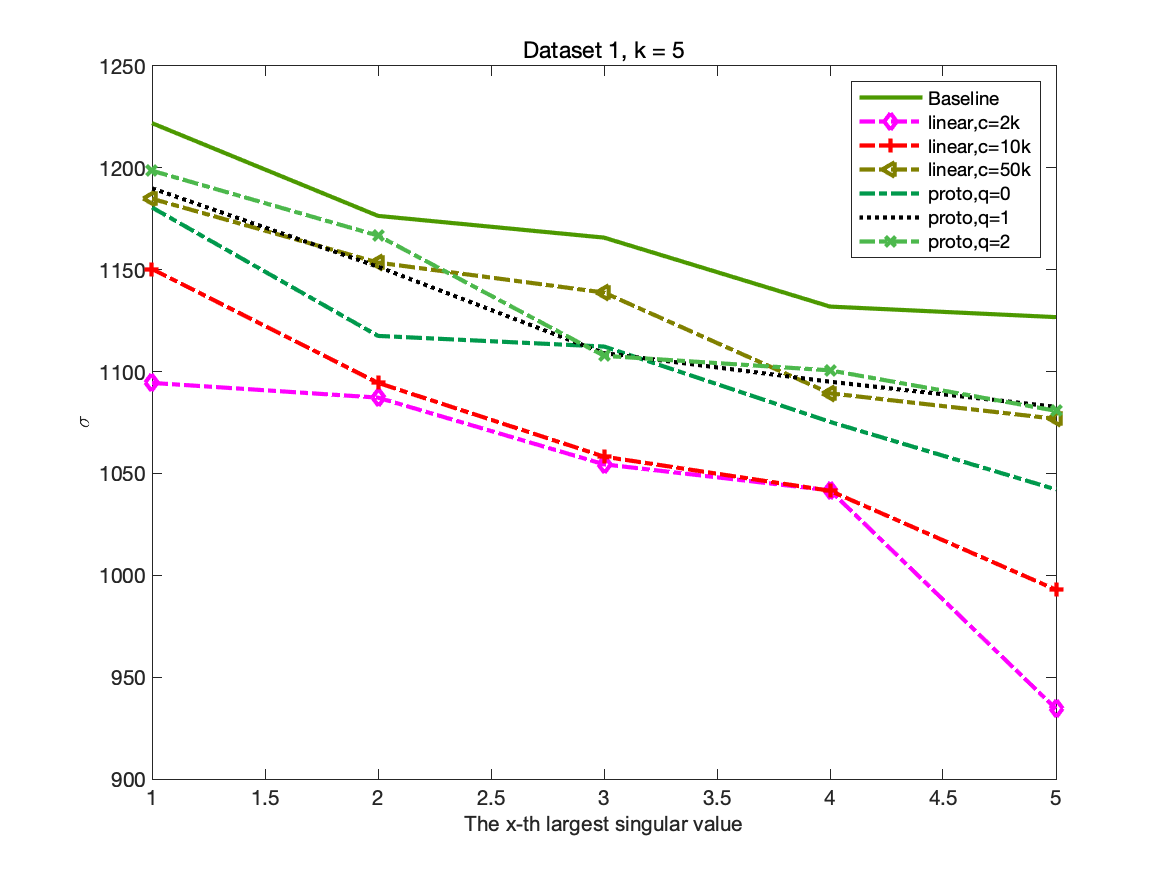
\includegraphics[width=1\linewidth]{./fig/dataset1_5.png}
		\caption{$k=5$}
	\end{minipage}
	\begin{minipage}{0.54\linewidth}
		\centering
		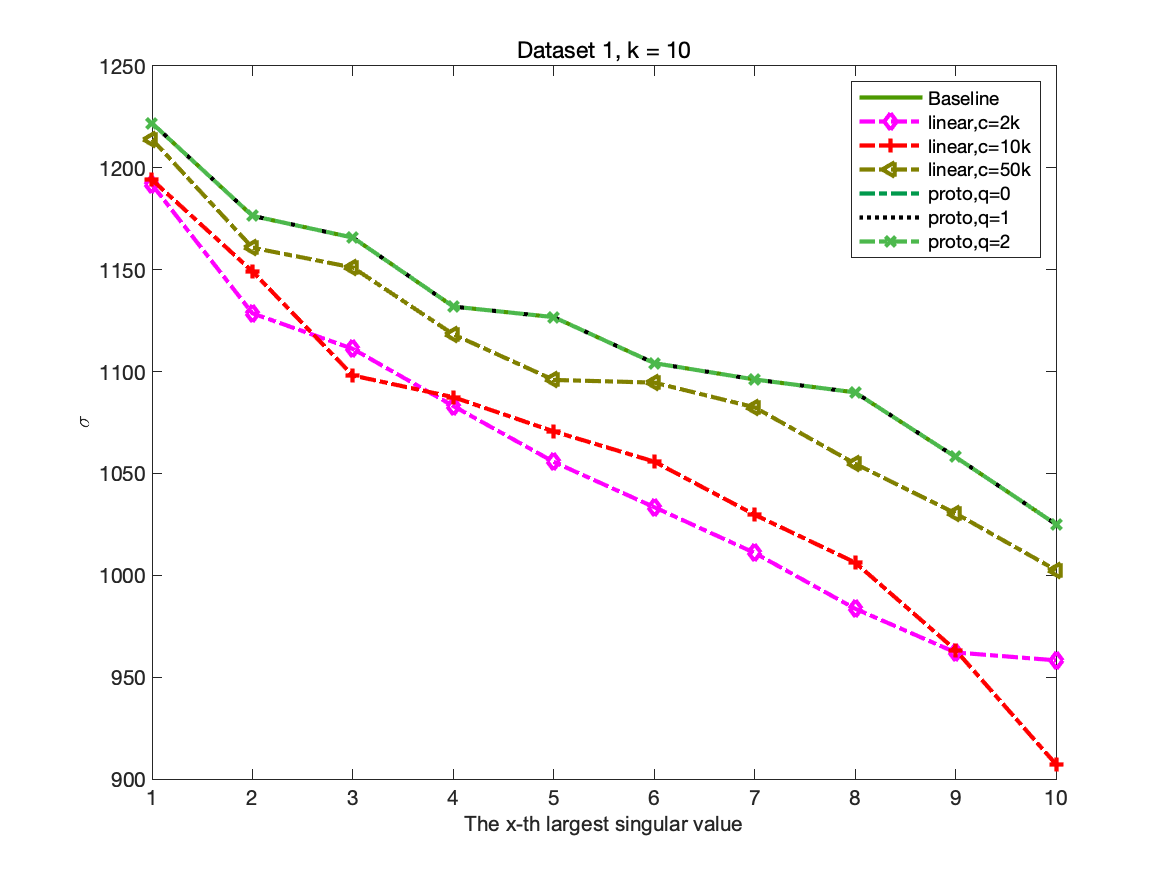
\includegraphics[width=1\linewidth]{./fig/dataset1_10.png}
		\caption{$k=10$}
	\end{minipage}
\end{figure} 

    \begin{figure}[p]
    \begin{minipage}{0.54\linewidth}
		\centering
		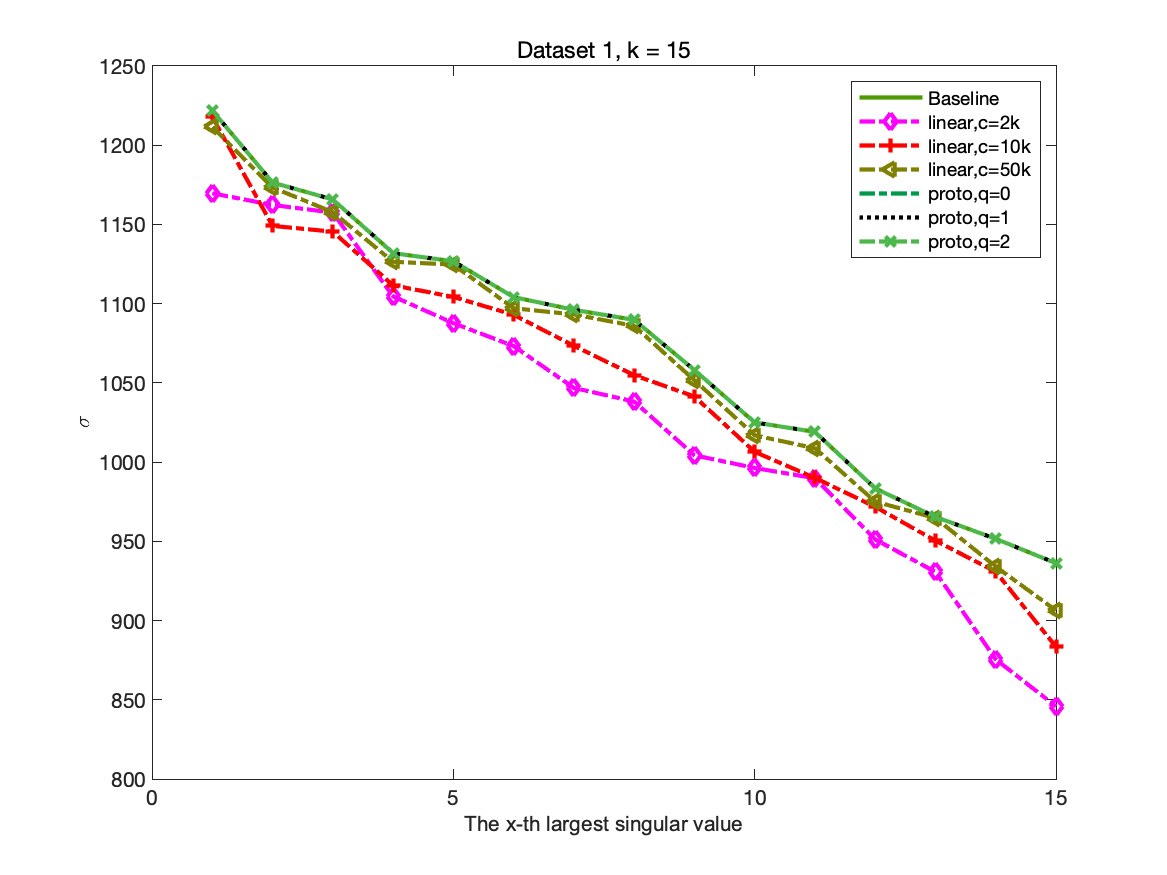
\includegraphics[width=1\linewidth]{./fig/dataset1_15.png}
		\caption{$k=15$}
	\end{minipage}
	\begin{minipage}{0.54\linewidth}
		\centering
		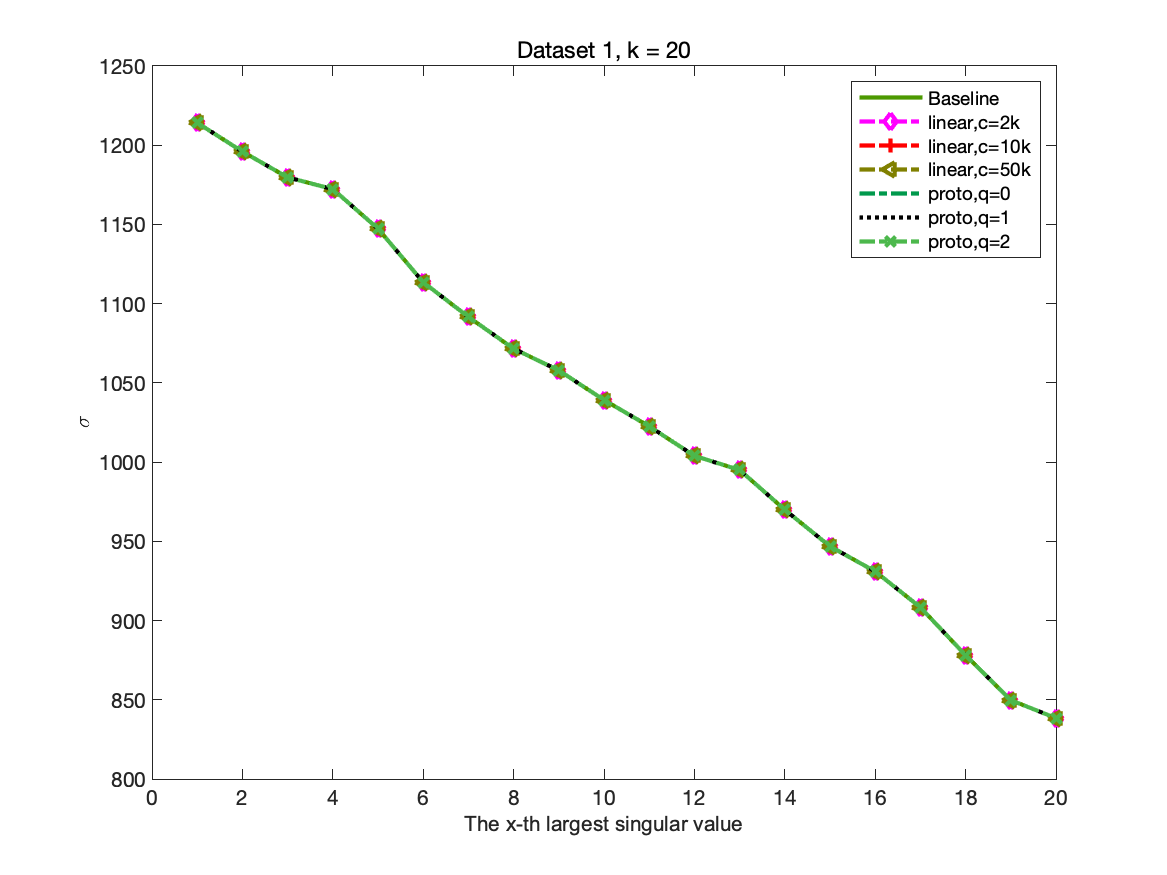
\includegraphics[width=1\linewidth]{./fig/dataset1_20.png}
		\caption{$k=20$}
	\end{minipage}
	\caption*{Results on dataset 1 with different $k$}
\end{figure}
\begin{table}\label{time1}
\centering
\begin{tabular}{|c|c|c|c|c|c|c|c|}

\hline
\multirow{2}{*}{ Algorithm} &\multicolumn{1}{c|}{baseline} &\multicolumn{3}{c|}{Linear time} &\multicolumn{3}{c|}{Prototype randomized}\\\cline{2-8}
 &- &$c=2k$ &$c=10k$ &$c=50k$ &$q=0$ &$q=1$ &$q=2$\\\hline
$k=5$ & $1.19e-02$ & $2.04e-02$ & $2.92e-02$ & $7.15e-02$ & $1.24e-01$ & $8.52e-02$ & $5.07e-02$\\\hline
$k=10$ & $1.69e-02$ & $1.78e-02$ & $5.79e-02$ & $1.45e-01$ & $1.94e-01$ & $1.33e-01$ & $4.16e-02$\\\hline
$k=15$ & $1.78e-02$ & $2.71e-02$ & $1.39e-01$ & $1.58e-01$ & $1.67e-01$ & $1.62e-01$ & $6.26e-02$\\\hline
$k=20$ & $2.02e-02$ & $3.79e-02$ & $1.81e-01$ & $1.75e-01$ & $1.92e-01$ & $1.78e-01$ & $7.03e-02$\\\hline
\end{tabular}
\caption{CPU time for Linear time SVD and Prototype randomized SVD with different parameters and $k$}
\end{table}

\begin{table}\label{sigma1}
\centering
\begin{tabular}{|c|c|c|c|c|c|c|}

\hline
\multirow{2}{*}{ Algorithm} &\multicolumn{3}{c|}{Linear time} &\multicolumn{3}{c|}{Prototype randomized}\\\cline{2-7}
 &$c=2k$ &$c=10k$ &$c=50k$ &$q=0$ &$q=1$ &$q=2$\\\hline
$k=5$ & $1.13e-01$ & $1.05e-01$ & $3.87e-02$ & $6.52e-02$ & $3.89e-02$ & $2.35e-02$\\\hline
$k=10$ & $7.22e-02$ & $4.76e-02$ & $2.56e-02$ & $7.99e-16$ & $8.29e-16$ & $8.48e-16$\\\hline
$k=15$ & $3.88e-02$ & $2.76e-02$ & $1.06e-02$ & $8.34e-16$ & $8.38e-16$ & $9.88e-16$\\\hline
$k=20$ & $8.49e-16$ & $8.40e-16$ & $7.33e-16$ & $8.84e-16$ & $6.73e-16$ & $1.09e-15$\\\hline
\end{tabular}
\caption{Relative error of eigenvalue for Linear time SVD and Prototype randomized SVD with different parameters and $k$ on dataset 1}
\end{table}

\begin{table}[H]\label{U1}
\centering
\begin{tabular}{|c|c|c|c|c|c|c|}

\hline
\multirow{2}{*}{ Algorithm} &\multicolumn{3}{c|}{Linear time} &\multicolumn{3}{c|}{Prototype randomized}\\\cline{2-7}
 &$c=2k$ &$c=10k$ &$c=50k$ &$q=0$ &$q=1$ &$q=2$\\\hline
$k=5$ & $1.31e-02$ & $1.27e-02$ & $9.22e-03$ & $1.19e-02$ & $1.05e-02$ & $6.48e-03$\\\hline
$k=10$ & $1.11e-02$ & $1.12e-02$ & $7.89e-03$ & $1.79e-15$ & $3.87e-15$ & $4.74e-15$\\\hline
$k=15$ & $1.11e-02$ & $1.04e-02$ & $6.10e-03$ & $1.46e-15$ & $1.14e-15$ & $1.93e-15$\\\hline
$k=20$ & $1.44e-15$ & $2.72e-15$ & $1.27e-15$ & $3.52e-15$ & $2.20e-15$ & $2.48e-15$\\\hline
\end{tabular}
\caption{Relative $\|\cdot\|_F$ error of $U$ for Linear time SVD and Prototype randomized SVD with different parameters and $k$ on dataset 1}
\end{table}

\begin{table}\label{V1}
\centering
\begin{tabular}{|c|c|c|c|c|c|c|}

\hline
\multirow{2}{*}{ Algorithm} &\multicolumn{3}{c|}{Linear time} &\multicolumn{3}{c|}{Prototype randomized}\\\cline{2-7}
 &$c=2k$ &$c=10k$ &$c=50k$ &$q=0$ &$q=1$ &$q=2$\\\hline
$k=5$ & $1.30e-02$ & $1.26e-02$ & $9.01e-03$ & $1.18e-02$ & $1.04e-02$ & $6.21e-03$\\\hline
$k=10$ & $1.09e-02$ & $1.11e-02$ & $7.71e-03$ & $1.80e-15$ & $3.88e-15$ & $4.73e-15$\\\hline
$k=15$ & $1.10e-02$ & $1.03e-02$ & $5.99e-03$ & $1.47e-15$ & $1.15e-15$ & $1.93e-15$\\\hline
$k=20$ & $1.44e-15$ & $2.72e-15$ & $1.28e-15$ & $3.52e-15$ & $2.20e-15$ & $2.48e-15$\\\hline
\end{tabular}
\caption{Relative $\|\cdot\|_F$ error of $V$ for Linear time SVD and Prototype randomized SVD with different parameters and $k$ on dataset 1}
\end{table}
  
\begin{figure}[p]
	\begin{minipage}{0.54\linewidth}
		\centering
		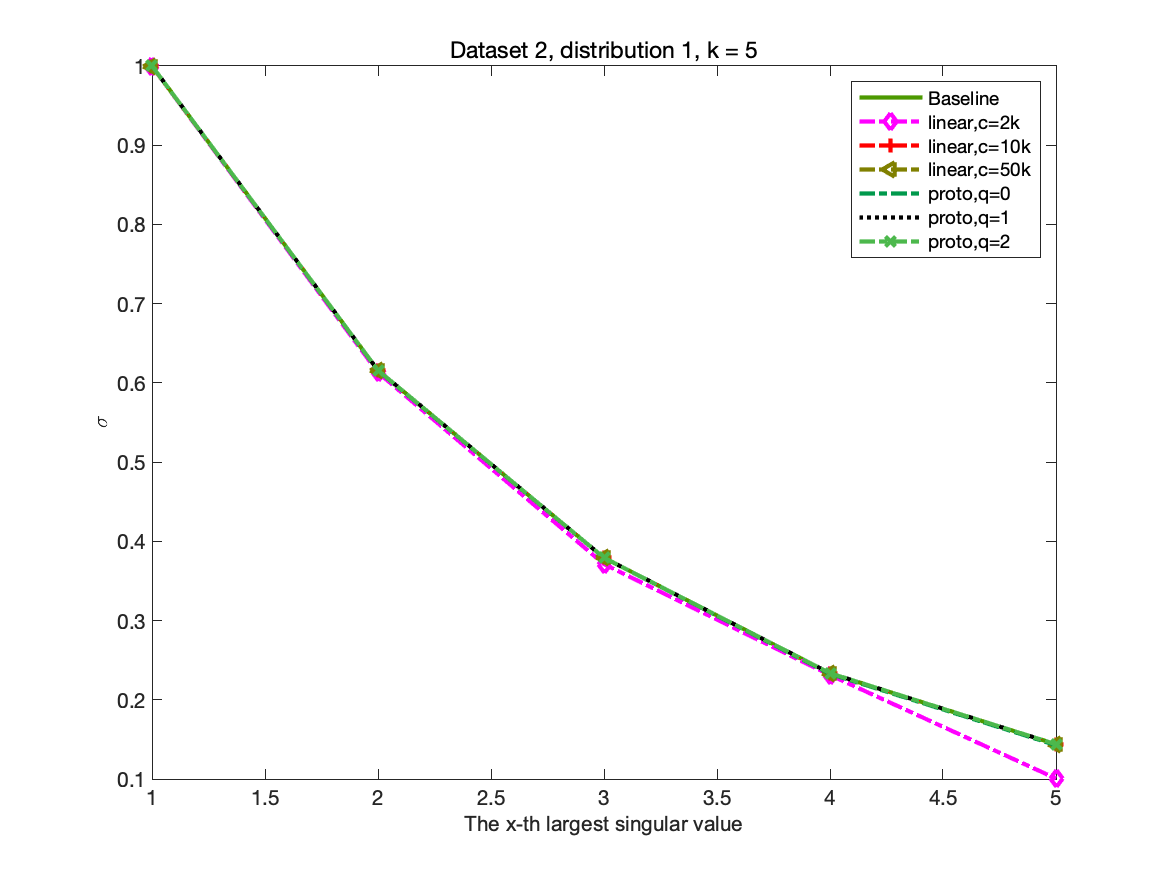
\includegraphics[width=1\linewidth]{./fig/dataset2_k5_t1.png}
		\caption{$k=5$}
	\end{minipage}
	\begin{minipage}{0.54\linewidth}
		\centering
		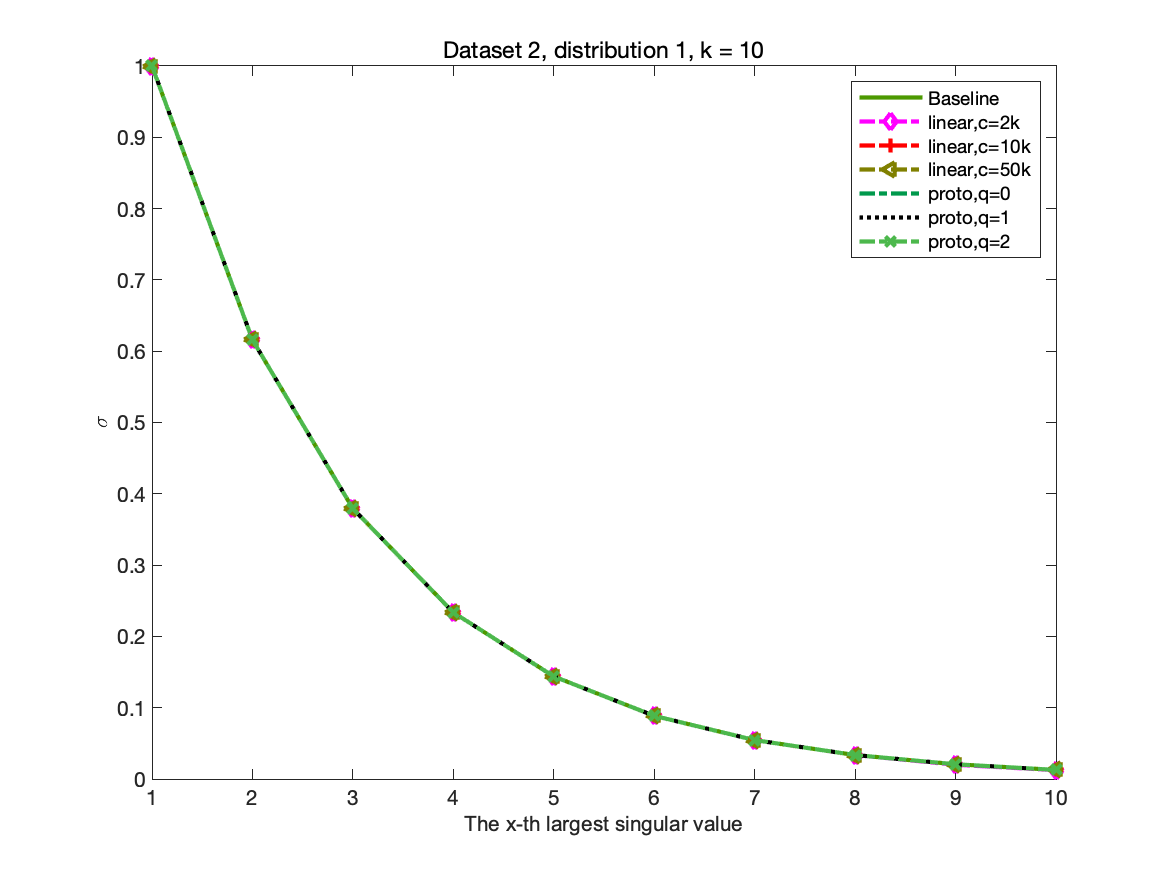
\includegraphics[width=1\linewidth]{./fig/dataset2_k10_t1.png}
		\caption{$k=10$}
	\end{minipage}
    \begin{minipage}{0.54\linewidth}
		\centering
		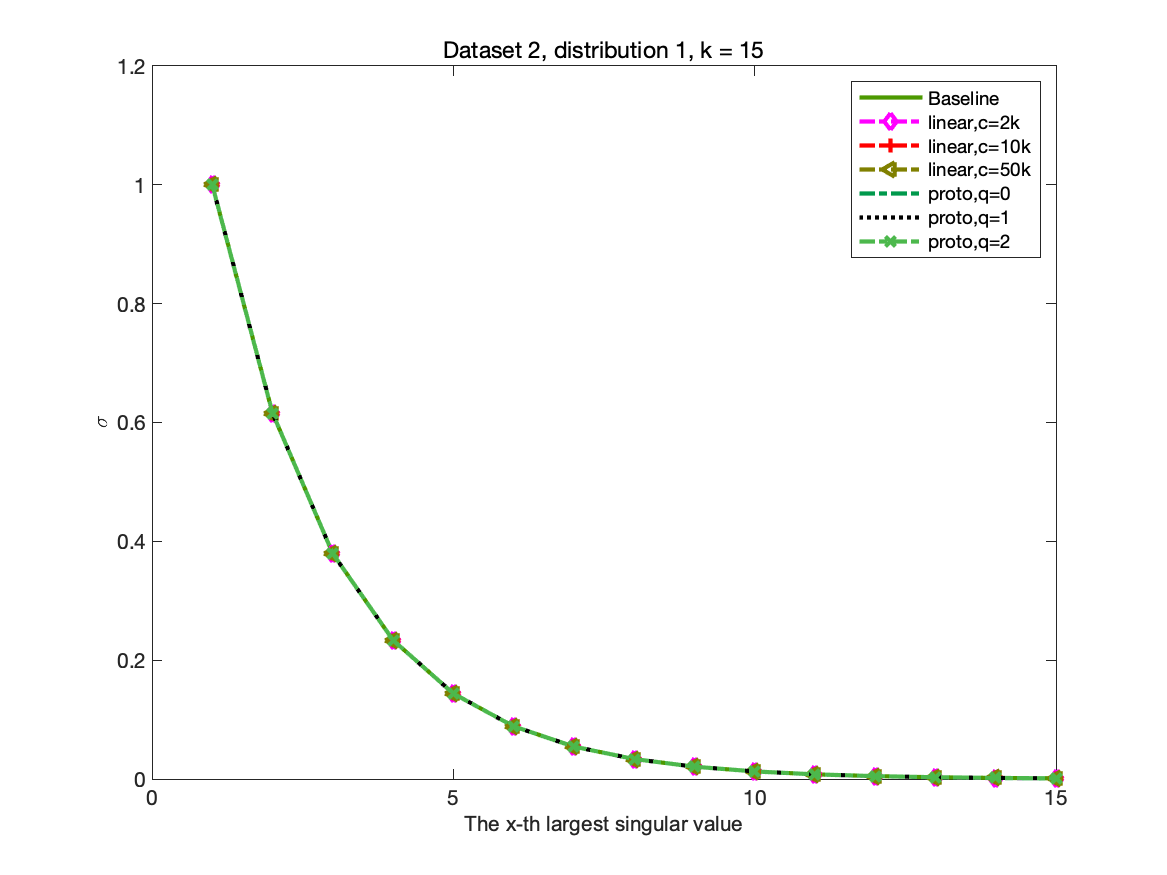
\includegraphics[width=1\linewidth]{./fig/dataset2_k15_t1.png}
		\caption{$k=15$}
	\end{minipage}
	\begin{minipage}{0.54\linewidth}
		\centering
		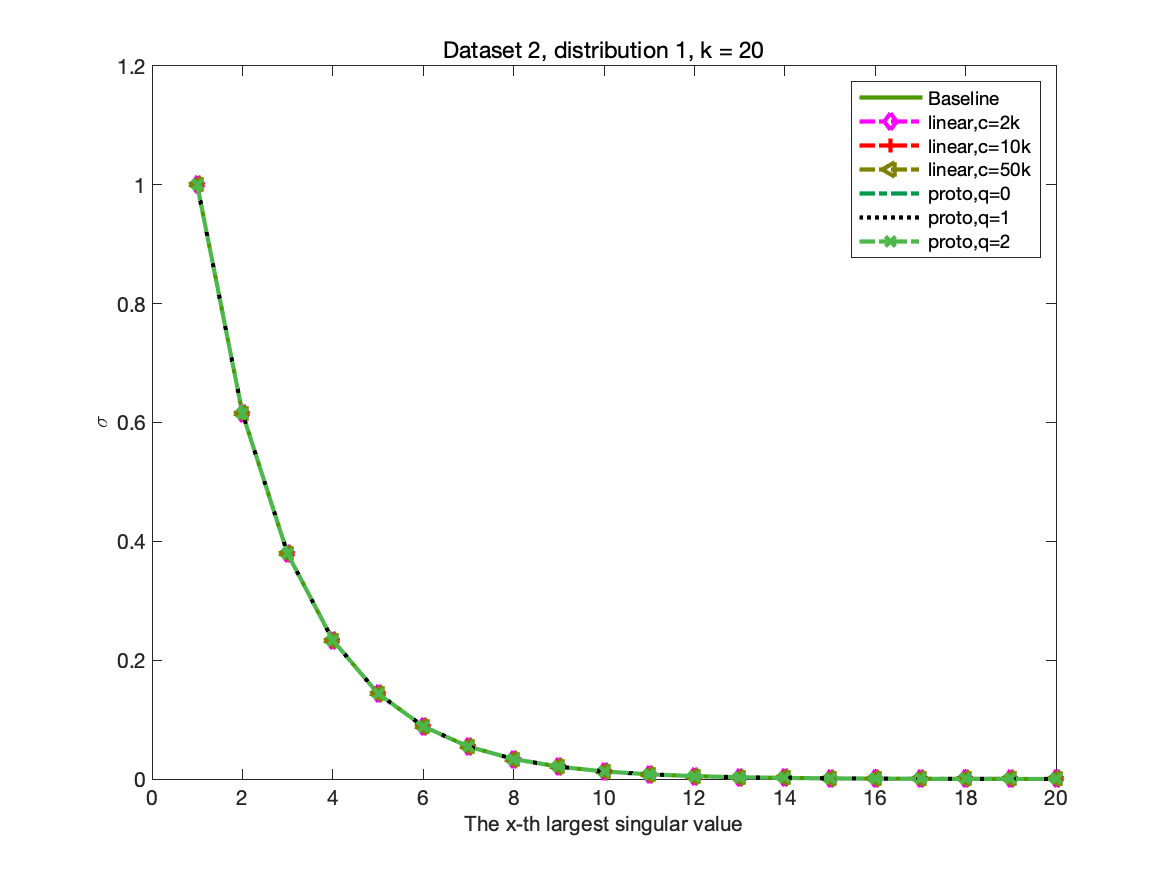
\includegraphics[width=1\linewidth]{./fig/dataset2_k20_t1.png}
		\caption{$k=20$}
	\end{minipage}
	\caption*{Results on dataset 2, distribution 1 with different $k$}
\end{figure} 
\begin{figure}[p]
	\begin{minipage}{0.54\linewidth}
		\centering
		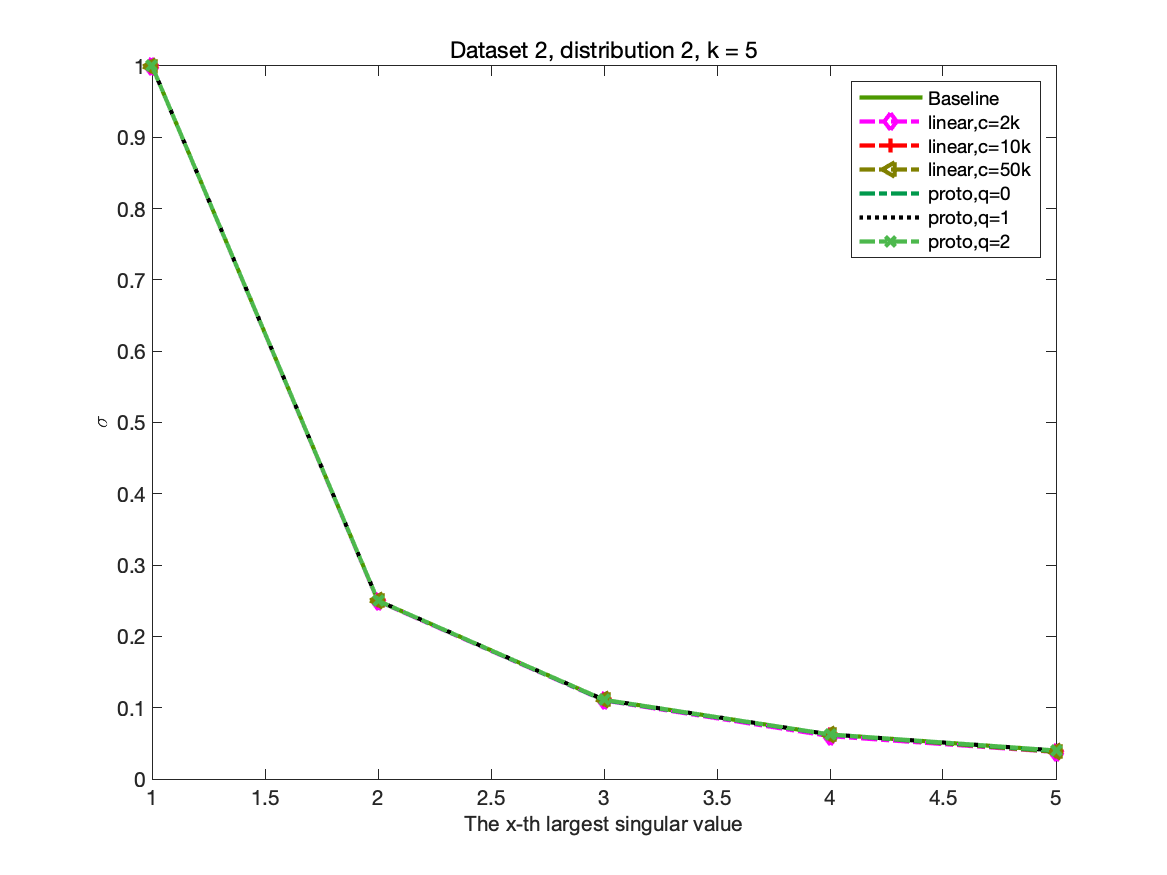
\includegraphics[width=1\linewidth]{./fig/dataset2_k5_t2.png}
		\caption{$k=5$}
	\end{minipage}
	\begin{minipage}{0.54\linewidth}
		\centering
		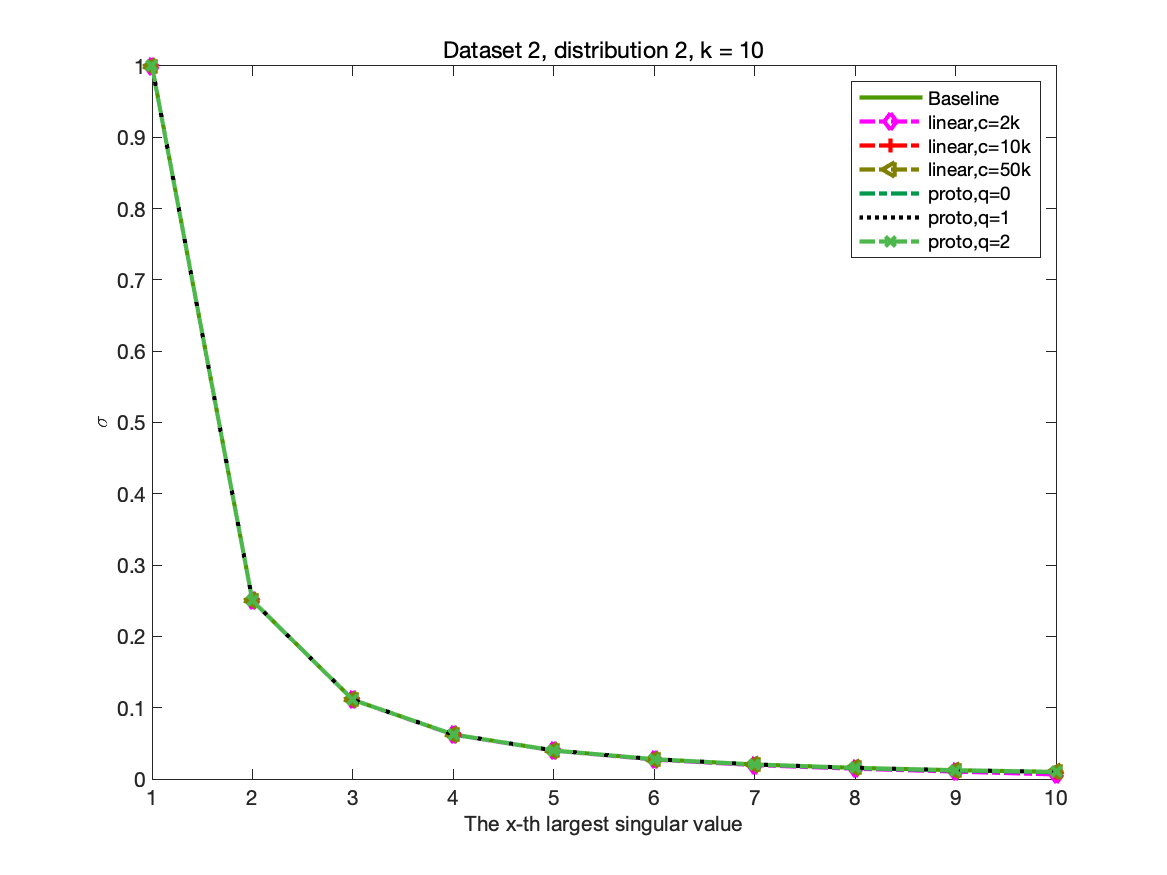
\includegraphics[width=1\linewidth]{./fig/dataset2_k10_t2.png}
		\caption{$k=10$}
	\end{minipage}
    \begin{minipage}{0.54\linewidth}
		\centering
		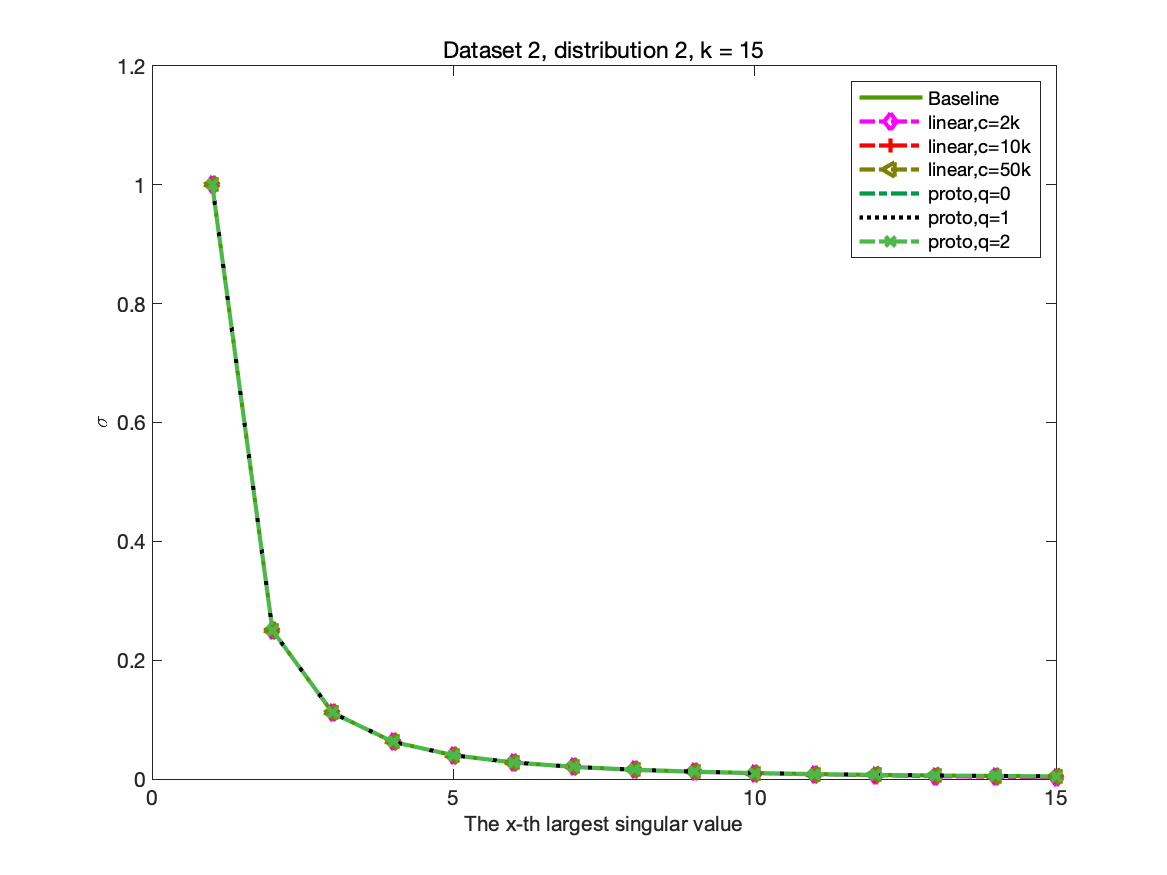
\includegraphics[width=1\linewidth]{./fig/dataset2_k15_t2.png}
		\caption{$k=15$}
	\end{minipage}
	\begin{minipage}{0.54\linewidth}
		\centering
		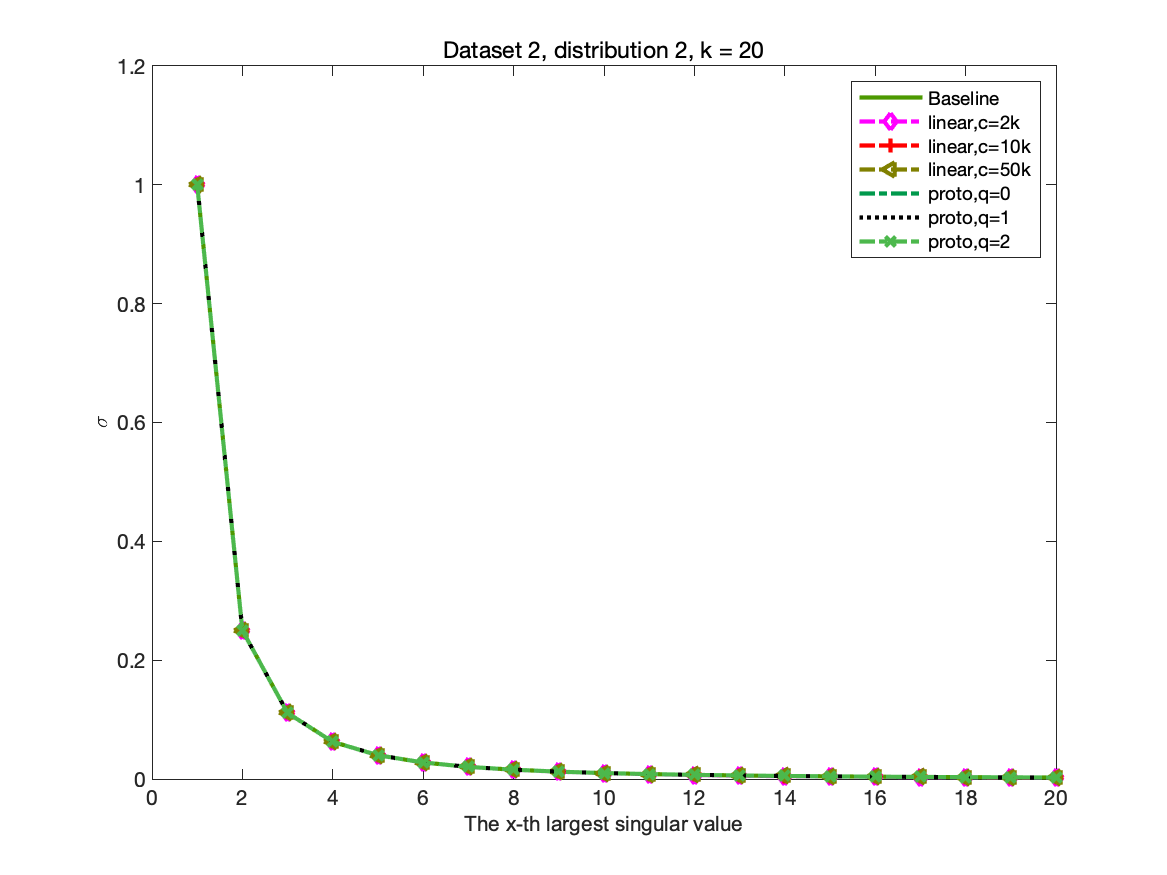
\includegraphics[width=1\linewidth]{./fig/dataset2_k20_t2.png}
		\caption{$k=20$}
	\end{minipage}
	\caption*{Results on dataset 2, distribution 1 with different $k$}
\end{figure} 
\begin{table}\label{time21}
\centering
\begin{tabular}{|c|c|c|c|c|c|c|c|}

\hline
\multirow{2}{*}{ Algorithm} &\multicolumn{1}{c|}{baseline} &\multicolumn{3}{c|}{Linear time} &\multicolumn{3}{c|}{Prototype randomized}\\\cline{2-8}
 &- &$c=2k$ &$c=10k$ &$c=50k$ &$q=0$ &$q=1$ &$q=2$\\\hline
$k=5$ & $1.07e+00$ & $1.16e+00$ & $1.13e+00$ & $2.48e-01$ & $7.98e-01$ & $7.77e-01$ & $2.03e-01$\\\hline
$k=10$ & $1.24e+00$ & $1.22e+00$ & $1.34e+00$ & $3.68e-01$ & $8.75e-01$ & $9.35e-01$ & $3.79e-01$\\\hline
$k=15$ & $1.47e+00$ & $1.47e+00$ & $1.75e+00$ & $5.26e-01$ & $1.32e+00$ & $1.35e+00$ & $6.82e-01$\\\hline
$k=20$ & $1.51e+00$ & $1.69e+00$ & $1.70e+00$ & $7.04e-01$ & $1.28e+00$ & $1.28e+00$ & $6.99e-01$\\\hline
\end{tabular}
\caption{CPU time for Linear time SVD and Prototype randomized SVD with different parameters and $k$}
\end{table}

\begin{table}\label{time22}
\centering
\begin{tabular}{|c|c|c|c|c|c|c|c|}

\hline
\multirow{2}{*}{ Algorithm} &\multicolumn{1}{c|}{baseline} &\multicolumn{3}{c|}{Linear time} &\multicolumn{3}{c|}{Prototype randomized}\\\cline{2-8}
 &- &$c=2k$ &$c=10k$ &$c=50k$ &$q=0$ &$q=1$ &$q=2$\\\hline
$k=5$ & $1.16e+00$ & $1.16e+00$ & $1.13e+00$ & $2.38e-01$ & $7.66e-01$ & $7.72e-01$ & $1.95e-01$\\\hline
$k=10$ & $1.27e+00$ & $1.21e+00$ & $1.25e+00$ & $3.81e-01$ & $9.73e-01$ & $9.70e-01$ & $3.96e-01$\\\hline
$k=15$ & $1.35e+00$ & $1.41e+00$ & $1.52e+00$ & $5.21e-01$ & $1.11e+00$ & $1.11e+00$ & $5.49e-01$\\\hline
$k=20$ & $1.37e+00$ & $1.54e+00$ & $1.71e+00$ & $6.81e-01$ & $1.35e+00$ & $1.22e+00$ & $6.84e-01$\\\hline
\end{tabular}
\caption{CPU time for Linear time SVD and Prototype randomized SVD with different parameters and $k$}
\end{table}

\begin{table}\label{sigma21}
\centering
\begin{tabular}{|c|c|c|c|c|c|c|}

\hline
\multirow{2}{*}{ Algorithm} &\multicolumn{3}{c|}{Linear time} &\multicolumn{3}{c|}{Prototype randomized}\\\cline{2-7}
 &$c=2k$ &$c=10k$ &$c=50k$ &$q=0$ &$q=1$ &$q=2$\\\hline
$k=5$ & $2.44e-02$ & $1.95e-03$ & $6.47e-04$ & $1.25e-04$ & $1.27e-08$ & $6.11e-14$\\\hline
$k=10$ & $2.64e-04$ & $1.31e-04$ & $2.20e-05$ & $5.00e-05$ & $1.56e-14$ & $5.59e-16$\\\hline
$k=15$ & $4.13e-04$ & $6.66e-05$ & $1.29e-05$ & $2.24e-04$ & $1.06e-09$ & $2.12e-07$\\\hline
$k=20$ & $3.57e-04$ & $2.19e-04$ & $1.06e-04$ & $3.03e-04$ & $2.37e-05$ & $2.31e-04$\\\hline
\end{tabular}
\caption{Relative error of eigenvalue for Linear time SVD and Prototype randomized SVD with different parameters and $k$ on dataset 2 with distribution 1}
\end{table}

\begin{table}\label{sigma22}
\centering
\begin{tabular}{|c|c|c|c|c|c|c|}

\hline
\multirow{2}{*}{ Algorithm} &\multicolumn{3}{c|}{Linear time} &\multicolumn{3}{c|}{Prototype randomized}\\\cline{2-7}
 &$c=2k$ &$c=10k$ &$c=50k$ &$q=0$ &$q=1$ &$q=2$\\\hline
$k=5$ & $6.24e-03$ & $2.44e-03$ & $8.57e-04$ & $3.59e-03$ & $1.53e-06$ & $1.28e-08$\\\hline
$k=10$ & $3.45e-03$ & $1.62e-03$ & $2.88e-04$ & $4.59e-04$ & $1.59e-06$ & $1.47e-09$\\\hline
$k=15$ & $1.75e-03$ & $2.79e-04$ & $5.37e-04$ & $2.60e-04$ & $3.27e-07$ & $1.40e-09$\\\hline
$k=20$ & $1.23e-03$ & $5.21e-04$ & $1.41e-04$ & $1.88e-04$ & $3.90e-07$ & $3.91e-09$\\\hline
\end{tabular}
\caption{Relative error of eigenvalue for Linear time SVD and Prototype randomized SVD with different parameters and $k$ on dataset 2 with distribution 2}
\end{table}

\begin{table}\label{U21}
\centering
\begin{tabular}{|c|c|c|c|c|c|c|}

\hline
\multirow{2}{*}{ Algorithm} &\multicolumn{3}{c|}{Linear time} &\multicolumn{3}{c|}{Prototype randomized}\\\cline{2-7}
 &$c=2k$ &$c=10k$ &$c=50k$ &$q=0$ &$q=1$ &$q=2$\\\hline
$k=5$ & $3.63e-03$ & $1.07e-03$ & $4.30e-04$ & $2.34e-04$ & $2.12e-06$ & $4.65e-09$\\\hline
$k=10$ & $8.07e-04$ & $6.64e-04$ & $1.78e-04$ & $3.50e-04$ & $5.90e-09$ & $5.84e-10$\\\hline
$k=15$ & $2.84e-03$ & $1.15e-03$ & $4.97e-04$ & $2.07e-03$ & $4.08e-06$ & $5.67e-05$\\\hline
$k=20$ & $6.30e-03$ & $5.64e-03$ & $4.72e-03$ & $5.75e-03$ & $3.16e-03$ & $5.63e-03$\\\hline
\end{tabular}
\caption{Relative $\|\cdot\|_F$ error of $U$ for Linear time SVD and Prototype randomized SVD with different parameters and $k$ on dataset 2 with distribution 1}
\end{table}

\begin{table}\label{U22}
\centering
\begin{tabular}{|c|c|c|c|c|c|c|}

\hline
\multirow{2}{*}{ Algorithm} &\multicolumn{3}{c|}{Linear time} &\multicolumn{3}{c|}{Prototype randomized}\\\cline{2-7}
 &$c=2k$ &$c=10k$ &$c=50k$ &$q=0$ &$q=1$ &$q=2$\\\hline
$k=5$ & $2.80e-03$ & $2.17e-03$ & $1.10e-03$ & $2.01e-03$ & $4.12e-05$ & $3.77e-06$\\\hline
$k=10$ & $4.93e-03$ & $3.64e-03$ & $1.17e-03$ & $1.31e-03$ & $7.05e-05$ & $1.98e-06$\\\hline
$k=15$ & $5.81e-03$ & $1.55e-03$ & $2.91e-03$ & $1.30e-03$ & $3.96e-05$ & $2.38e-06$\\\hline
$k=20$ & $5.81e-03$ & $4.73e-03$ & $1.44e-03$ & $1.37e-03$ & $5.22e-05$ & $4.69e-06$\\\hline
\end{tabular}
\caption{Relative $\|\cdot\|_F$ error of $U$ for Linear time SVD and Prototype randomized SVD with different parameters and $k$ on dataset 2 with distribution 2}
\end{table}

\begin{table}\label{V21}
\centering
\begin{tabular}{|c|c|c|c|c|c|c|}

\hline
\multirow{2}{*}{ Algorithm} &\multicolumn{3}{c|}{Linear time} &\multicolumn{3}{c|}{Prototype randomized}\\\cline{2-7}
 &$c=2k$ &$c=10k$ &$c=50k$ &$q=0$ &$q=1$ &$q=2$\\\hline
$k=5$ & $2.02e-03$ & $6.35e-04$ & $1.45e-04$ & $1.88e-05$ & $1.21e-07$ & $2.57e-10$\\\hline
$k=10$ & $2.49e-04$ & $3.59e-04$ & $4.65e-05$ & $1.96e-05$ & $2.99e-11$ & $8.94e-12$\\\hline
$k=15$ & $7.72e-04$ & $2.90e-04$ & $3.74e-05$ & $1.95e-04$ & $2.03e-07$ & $5.80e-06$\\\hline
$k=20$ & $4.82e-03$ & $4.45e-03$ & $4.33e-03$ & $3.74e-03$ & $3.01e-03$ & $4.60e-03$\\\hline
\end{tabular}
\caption{Relative $\|\cdot\|_F$ error of $V$ for Linear time SVD and Prototype randomized SVD with different parameters and $k$ on dataset 2 with distribution 1}
\end{table}

\begin{table}\label{V22}
\centering
\begin{tabular}{|c|c|c|c|c|c|c|}

\hline
\multirow{2}{*}{ Algorithm} &\multicolumn{3}{c|}{Linear time} &\multicolumn{3}{c|}{Prototype randomized}\\\cline{2-7}
 &$c=2k$ &$c=10k$ &$c=50k$ &$q=0$ &$q=1$ &$q=2$\\\hline
$k=5$ & $8.59e-04$ & $1.35e-03$ & $5.10e-04$ & $4.77e-04$ & $8.59e-06$ & $9.38e-07$\\\hline
$k=10$ & $4.51e-03$ & $3.27e-03$ & $6.96e-04$ & $5.06e-04$ & $1.96e-05$ & $4.43e-07$\\\hline
$k=15$ & $5.37e-03$ & $9.52e-04$ & $2.66e-03$ & $4.98e-04$ & $9.63e-06$ & $4.68e-07$\\\hline
$k=20$ & $5.32e-03$ & $4.53e-03$ & $1.05e-03$ & $5.52e-04$ & $1.18e-05$ & $1.18e-06$\\\hline
\end{tabular}
\caption{Relative $\|\cdot\|_F$ error of $V$ for Linear time SVD and Prototype randomized SVD with different parameters and $k$ on dataset 2 with distribution 2}
\end{table}


We observe that the Linear time SVD works not very well on dataset 1 when $c$ is small, however, it shows good performance when $k$ or $c$ is large. Both algorithms behave well on dataset 2, from that the tables show that they can exactly recover the eigenvalues even when $k=5$. An explanation for better behavior when $k$ is larger is that larger $k$ results in larger sample sets, which leads to better simulation of $A$. Another interpretation is that the rank of $A$ is exactly $20$ in the first dataset, thus when $k\ge 10$, the restoration of the information of $A$ is complete for the Prototype SVD and $k=20$ for Linear time SVD.

On the other hand, we find that for problems of small scale (rank) like dataset 1, the random SVD has little advantage, while for much larger matrix in dataset 2, the random algorithms outperform the baseline MATLAB SVD, which is corresponding to our intuition that, it is hard to defeat MATLAB when the problem is of small scale, while we can do much better for larger problem.
\bibliographystyle{plain}  
\bibliography{ref}
\end{document}